\documentclass[11pt, letterpaper, twocolumn, fleqn]{article}
\usepackage[margin=0.5in]{geometry}
\usepackage{amssymb}
\usepackage{amsmath}
\usepackage{graphicx}
\graphicspath{ {./images/} }

\let\oldemptyset\emptyset
\let\emptyset\varnothing

\begin{document}
    \paragraph{3.1.1} 
    \renewcommand{\labelenumi}{\alph{enumi}.}
    \begin{enumerate}
        \item True
        \item False
        \item True  
        \addtocounter{enumi}{2}
        \item False
        \item True
    \end{enumerate}
    
    \paragraph{3.1.3}
    \renewcommand{\labelenumi}{\alph{enumi}.}
    \begin{enumerate}
        \item True
        \item True
        \item False
    \end{enumerate}
    
    \paragraph{3.1.6}
    \renewcommand{\labelenumi}{\alph{enumi}.}
    \begin{enumerate}
        \item False
        \item True
        \item True
        \item False
        \item True
    \end{enumerate}
    
    \paragraph{3.2.1}
    \renewcommand{\labelenumi}{\alph{enumi}.}
    \begin{enumerate}
        \item True
        \item True
        \item False
        \addtocounter{enumi}{1}
        \item True
        \item True
        \addtocounter{enumi}{3}
        \item False
        \item False
    \end{enumerate}
    
    \paragraph{3.2.2}
    \renewcommand{\labelenumi}{\alph{enumi}.}
    \begin{enumerate}
        \item $\{\emptyset, \{a\}\}$
        \item $\{\emptyset, \{1\},\{2\},\{1,2\}\}$
    \end{enumerate}
    
    \paragraph{3.3.1}
    \renewcommand{\labelenumi}{\alph{enumi}.}
    \begin{enumerate}
        \item $\{-3, 0, 1, 4, 17, -12, -5, 1, 4, 6\}$
        \item $\{1,4\}$
        \addtocounter{enumi}{3}
        \item $\{-3,1,17\}$
        \addtocounter{enumi}{1}
        \item $\{-3,0,1,4,17\}$
    \end{enumerate}
    
    \paragraph{3.3.3}
    $\{1,2,4\},\{1,3,9\},\{1,4,16\},\{1,5,25\}$
    
    \renewcommand{\labelenumi}{\alph{enumi}.}
    \begin{enumerate}
        \item $\{1\}$
        \item $\{1, 2, 3, 4, 5, 9, 16, 25\}$
    \end{enumerate}
    
    \paragraph{3.4.1}
    \renewcommand{\labelenumi}{\alph{enumi}.}
    \begin{enumerate}
        \item Let $A = \{1,2,3\}$, $B = \{2,3,4\}$, and $C = \{3,4,5\}$. 
        
        $$
            A-(B-C) = \{1,3\}
        $$
        $$
            (A-B)-C = \{1\}
        $$
        
        Therfore $A-(B-C) \neq (A-B)-C$
    \end{enumerate}
    
    \paragraph{3.5.1}
    \renewcommand{\labelenumi}{\alph{enumi}.}
    \begin{enumerate}
        \item Complement
        \addtocounter{enumi}{1}
        \item De Morgan's 
    \end{enumerate}
    
    \paragraph{3.5.2}
    \renewcommand{\labelenumi}{\alph{enumi}.}
    \begin{enumerate}
        \item 
            \begin{align*}
                C   & = (\bar{A} \cap C) \cup (A \cap C)    \\
                    & = (C \cap \bar{A}) \cup (C \cap A)    \tag{Commutative} \\
                    & = C \cap (\bar{A} \cup A)             \tag{Distributive} \\
                    & = C \cap U                            \tag{Complement} \\
                    & = C                                   \tag{Identity}
            \end{align*}
        \item
            \begin{align*}
                A   &= (B \cup A) \cap (\bar{B} \cup A ))   \\
                    &= ((A \cup B) \cap (A \cup \bar{B}))   \tag{Commutative}\\
                    &= A \cup (B \cap \bar{B})              \tag{Distributive}\\
                    &= A \cup \emptyset                     \tag{Complement}\\
                    &= A                                    \tag{Identity}
            \end{align*}
        \addtocounter{enumi}{1}
        \item
            \begin{align*}
                \bar{A} \cap B &= \bar{A} \cap (A \cup B) \\
                               &=((\bar{A} \cap A)\cup(\bar{A} \cap B)) \tag{Distributive}\\
                               &=(\emptyset \cup (\bar{A} \cap B))      \tag{Complement}\\
                               &=\bar{A} \cap B                         \tag{Identity}
            \end{align*}
        \addtocounter{enumi}{2}
        \item
            \begin{align*}
                U &= A \cup (B \cup \bar{B})    \\
                  &= A \cup U   \tag{Complement}\\
                  &= U          \tag{Domination}
            \end{align*}
    \end{enumerate}
    
    \paragraph{3.6.1}
    \renewcommand{\labelenumi}{\alph{enumi}.}
    \begin{enumerate}
        \item (tall, no-foam, whole)
        \item (foam, grande, non-fat)
        \item \{(foam, non-fat),(foam, whole),(no-foam, non-fat),(no-foam, whole)\}
    \end{enumerate}
    
    \paragraph{3.6.3}
    \renewcommand{\labelenumi}{\alph{enumi}.}
    \begin{enumerate}
        \item False
        \item True
    \end{enumerate}
    
    \paragraph{3.6.4}
    \renewcommand{\labelenumi}{\alph{enumi}.}
    \begin{enumerate}
        \item \{(++),(+-),(-+),(--)\} 
        \item \{(000),(001),(010),(011),(100),(101),(110),(111)\}
    \end{enumerate}
    
    \paragraph{3.7.1}
    \renewcommand{\labelenumi}{\alph{enumi}.}
    \begin{enumerate}
        \item They do not form a partition. Since $2 \in A$ and $2 \in B$, A and B are not mutually disjoint. Therfore they do not form a partition of the set D.
        \item They do not form a partition. $D \neq B \cup C = \{2,3,4,5\}$ because $\{1, 6\} \notin B \cup C$. 
    \end{enumerate}
    
    \paragraph{3.7.2}
    \renewcommand{\labelenumi}{\alph{enumi}.}
    \begin{enumerate}
        \item 
            First Partition = C,E \newline
            Second Partition = E,D,F
    \end{enumerate}
    
    \paragraph{3.8.1}
    \renewcommand{\labelenumi}{\alph{enumi}.}
    \begin{enumerate}
        \item The domain of f is \{a,b,c,d,e\}
        \item The target of f is \{w,x,y,z\}
        \item The range of f is \{w,y,z\}
    \end{enumerate}
    
    \paragraph{3.8.4}
    \renewcommand{\labelenumi}{\alph{enumi}.}
    \begin{enumerate}
        \item The domain of f is \{(0,0),(0,1),(1,0),(1,1)\}
        \item 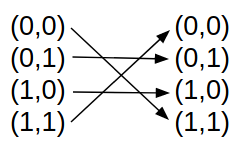
\includegraphics[scale=.5]{384b}
    \end{enumerate}
    
    \paragraph{3.8.5}
    \renewcommand{\labelenumi}{\alph{enumi}.}
    \begin{enumerate}
        \item \{3,5,7,9\}
        \item \{4,9,16,25\}
        \item \{0,1,2\}
        \addtocounter{enumi}{4}
        \item \{(1,1),(1,2),(1,3),(2,1),(2,2),(2,3),(3,1),(3,2),(3,3)\}
        \item \{(1,2),(1,3),(1,4),(2,2),(2,3),(2,4),(3,2),(3,3),(3,4)\}
    \end{enumerate}
    
    \paragraph{3.9.3}
    \renewcommand{\labelenumi}{\alph{enumi}.}
    \begin{enumerate}
        \item $\lfloor -3.7 \rfloor = -4$
        \item $\lceil -4.2 \rceil = -4$
        \item $\lceil 5 \rceil = 5$
        \item $\lfloor \lfloor 3.5 \rfloor - 4.3\rfloor = \lfloor 3 - 4.3 \rfloor = -2 $
        \item $\lfloor \frac{3}{2} + \lceil \frac{1}{3} \rceil \rfloor = \lfloor \frac{3}{2} + 1 \rfloor = 2$
    \end{enumerate}
    
    \paragraph{3.9.4}
    \renewcommand{\labelenumi}{\alph{enumi}.}
    \begin{enumerate}
        \item 
            True. Since an even integer n can be represented with $n = 2k$ for some integer k, we can substitute this into the given equation. 
            \begin{align*}
                \lfloor \frac{n}{2} \rfloor &= \frac{n}{2} \\
                \lfloor \frac{2k}{2} \rfloor &= \frac{2k}{2} \\
                \lfloor k \rfloor &= k
            \end{align*}
            Since k is an integer and the floor of any integer is equal to that integer, and $\lfloor \frac{n}{2} \rfloor = \frac{n}{2}$ can be represented by $\lfloor k \rfloor = k$, then if n is an even integer then $\lfloor \frac{n}{2} \rfloor = \frac{n}{2}$.
        \item 
            True. Since an odd integer n can be represented with $n = 2k-1$ for some integer k, we can substitue this into the given equation.
            \begin{align*}
                \lfloor \frac{n}{2} \rfloor     &= \frac{n-1}{2} \\
                \lfloor \frac{2k-1}{2} \rfloor  &= \frac{2k-1-1}{2} \\
                \lfloor k - \frac{1}{2} \rfloor &= k-1 \\
            \end{align*}
            Since k is an integer, $\lfloor k - \frac{1}{2} \rfloor$ will always round down to the next lowest integer. In other words it must equal $k-1$. Since $\lfloor \frac{n}{2} \rfloor = \frac{n-1}{2}$ can be represented by $\lfloor k - \frac{1}{2} \rfloor = k-1$, then $\lfloor \frac{n}{2} \rfloor = \frac{n-1}{2}$ must be true for some odd integer n.
    \end{enumerate}
    
    \paragraph{3.10.1}
    \renewcommand{\labelenumi}{\alph{enumi}.}
    \begin{enumerate}
        \item Not onto. $f(x,y)=2x-4y=2(x-2y)=2k$ where $k=x-2y$. Since x and y are integers, k is also an integer. Since $f(x,y)$ can be represented by the equation for an even number, then $f(x,y)$ does not map odd numbers. Therefore $f(x,y)$ is not onto.
        \item Onto. \newline
        Case 1: To obtain any negative integer v, set $x = 0$ and $y = v$. \newline
        Case 2: To obtain any positive integer w, set $x=w$ and $y = 0$. \newline
        Case 3: To obtain 0, set $y=x=0$
    \end{enumerate}
    
    \paragraph{3.10.2}
    \renewcommand{\labelenumi}{\alph{enumi}.}
    \begin{enumerate}
        \item Not one-to-one because $f(1)=(1)^2=1$ and $f(-1)=(-1)^2=1$. \newline
        Not onto because a real number squared can never be negative.
        \item Onto and one-to-one.
        \item Not onto. For example, no integer x exists such that $h(x)=x^3=2$. One-to-one.
        \addtocounter{enumi}{2}
        \item Onto and one-to-one
        \addtocounter{enumi}{3}
        \item Onto and one-to-one
    \end{enumerate}
    
    \paragraph{3.11.1}
    \renewcommand{\labelenumi}{\alph{enumi}.}
    \begin{enumerate}
        \item $f^{-1}$ is not well defined because $f^{-1}(w) = d$ and $f^{-1}(w) = b$
        \item 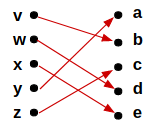
\includegraphics{3111b}
        \item $f^{-1}$ is not well defined because $f^{-1}(y)$ is not defined.
    \end{enumerate}
    
    \paragraph{3.11.2}
    \renewcommand{\labelenumi}{\alph{enumi}.}
    \begin{enumerate}
        \item $f^{-1}$ is well defined. $f^{-1}(x)=x-3$
        \item Because there is no integer x such that $f(x)=2x+34=3$, $f(x)$ is not onto. Therfore $f^{-1}$ is not well defined.
        \addtocounter{enumi}{3}
        \item $f(001)=f(101)=101$, therfore $f(x)$ is not one-to-one. Also there is no x such that $f(x)=000$, therfore $f(x)$ is not onto. Since $f(x)$ is neither one-to-one nor onto, $f^{-1}$ is not well defined.
    \end{enumerate}
    
    \paragraph{3.12.2}
    \renewcommand{\labelenumi}{\alph{enumi}.}
    \begin{enumerate}
        \item $(f \circ g)(0)=(2^{(0)})^2=1^2=1$ 
        \item $(f \circ h)(52)=(\lceil \frac{(52)}{5} \rceil)^2 = (11)^2 = 121$
        \item 
            \begin{align*}
                (g \circ h \circ f)(4) &= 2^{\lceil \frac{(4)^2}{5} \rceil} \\
                                       &= 2^{\lceil \frac{16}{5} \rceil} \\
                                       &= 2^{4} \\
                                       &= 16
            \end{align*}
        \addtocounter{enumi}{1}
        \item $(f \circ g)(x)=(2^x)^2 = 2^{2x}$
    \end{enumerate}
    
    \paragraph{3.12.5}
    \renewcommand{\labelenumi}{\alph{enumi}.}
    \begin{enumerate}
        \item The range of g is \{2, 3\}
        \item The domain of $h \circ g$ is \{a, b, c\}
        \item $h^{-1}(y) = 3$
        \item The domain of of $h^{-1} \circ h$ is \{1, 2, 3, 4\}
        \item $(h \circ g)(b)=w$
    \end{enumerate}
\end{document}          
